\section{Experiments}

In this section, we demonstrate the performance of \dataname by performing supervised fine-tuning (SFT) on baseline models of different sizes. We then compare the fine-tuned models' performance against existing model baselines across several widely used agentic tool-call benchmarks.

\subsection{Experiment Setup}

\textbf{Model and Baseline Setup.} We perform supervised fine-tuning on \texttt{Qwen2.5-7B-Instruct}, \texttt{Qwen2.5-14B-Instruct}, and \texttt{Qwen2.5-32B-Instruct} \citep{qwen2.5} to demonstrate the efficacy of \dataname across models of varying sizes. Detailed fine-tuning parameters are provided in Appendix \ref{app:fine-tune-parameter}. We benchmark the performance of our fine-tuned models against models of comparable or larger scales, including \texttt{DeepSeek-V3} \cite{deepseekai2025deepseekv3technicalreport}, \texttt{Qwen2.5-72B-Instruct}, \texttt{Qwen3-235B-A22B}, \texttt{Qwen3-32B} \cite{yang2025qwen3technicalreport}, and closed-source OpenAI models such as o3-mini, GPT-4.1, and GPT-4.5-Preview.

\begin{table}[t!]
  \vspace{-1em}
  \centering
  \caption{This table compares the performance of \datanamen-tuned models and baselines on the BFCL-V3 benchmark. We observe that \dataname remarkably improves baseline model performance through supervised fine-tuning (SFT) and enables smaller models to outperform larger models across different evaluation aspects.}
  % \vspace{-1.5em}
  \label{tab:bfclv3-results-table}
  \resizebox{\textwidth}{!}{%
\begin{tabular}{@{}lcccccc@{}}
\toprule
\textbf{Model}                          & \textbf{Overall} & \multicolumn{2}{c}{\textbf{Single Turn}} & \textbf{Multi Turn} & \multicolumn{2}{c}{\textbf{Hallucination}} \\
                                       \cmidrule(lr){2-2} \cmidrule(lr){3-4} \cmidrule(lr){5-5} \cmidrule(lr){6-7}
                                       &                  & \textit{Non-live (AST)}        & \textit{Live (AST)}       &                     & \textit{Relevance}           & \textit{Irrelevance}         \\
\midrule  
DeepSeek-V3                            & 64.71\%          & 88.54\%               & 77.34\%          & 29.87\%             & \textbf{83.33\%}             & 76.49\%              \\
Qwen2.5-72B-Instruct              & 64.37\%          & 87.56\%               & 78.68\%          & 29.38\%             & 72.22\%             & 77.41\%              \\
Qwen3-235B-A22B                        & 67.94\%          & 87.90\%               & 77.03\%          & 40.12\%             & \textbf{83.33\% }            & 76.32\%              \\
Qwen3-32B                              & 69.25\%          & \textbf{88.90\%}               & 77.83\%          & 43.12\%             & 72.22\%             & 75.79\%  \\
% ToolACE-2-8B &  68.73\% & 87.58\%   & 80.05\% & 37.00\% & 72.22\% & 90.11\% \\
% xLAM-2-70b-fc-r (FC)                   & 78.45\%          & 88.44\%               & 72.95\%          & 75.00\%           & 66.67\%               & 78.91\%\\
o3-Mini                                & 64.61\%          & 86.15\%               & 79.08\%          & 28.75\%             & 72.22\%             & 82.96\%              \\
GPT-4.1                                & 68.69\%          & 85.42\%               & \textbf{79.92\%}          & 40.50\%             & 77.78\%             & \textbf{85.95\%}              \\
GPT-4.5-Preview                        & 70.32\%          & 86.12\%               & 79.34\%          & 45.38\%             & 66.67\%             & 83.64\%              \\
\midrule
\midrule
%\cmidrule{1-1} \cmidrule(lr){2-2} \cmidrule(lr){3-4} \cmidrule(lr){5-5} \cmidrule{6-7}
Qwen2.5-7B-Instruct               & 55.10\%          & 84.19\%               & 72.32\%          & 12.88\%             & 72.22\%             & 67.93\%              \\
\quad\textit{with \dataname}  & \withsup{58.26\%}{3.16} & 78.52\%               & 74.50\%          & 22.62\%             & 66.67\%             & 75.18\%              \\
\midrule
Qwen2.5-14B-Instruct              & 57.69\%          & 83.38\%               & 73.70\%          & 19.75\%             & \textbf{83.33\%}             & 68.46\%              \\
\quad\textit{with \dataname} & \withsup{65.09\%}{7.40} & 85.42\%               & 76.01\%          & 35.25\%             & 72.22\%             & 75.96\%              \\
\midrule
Qwen2.5-32B-Instruct              & 61.73\%          & 85.58\%               & 76.01\%          & 26.38\%             & 72.22\%             & 72.68\%              \\
\quad\textit{with \dataname} & \withsup{\textbf{70.45\%}}{8.72} & 87.12\%               & 78.90\%          & \textbf{46.50\%}             & 77.78\%             & 78.10\%              \\
\bottomrule
\end{tabular}
\vspace{-3em}
}
\end{table}

\textbf{\dataname Setup.} Given the large volume of the full dataset, we adopted a strategy similar to \cite{Xu2025KodCodeAD} by sampling from a high-quality subset of \datanamen. This subset was selected based on the following criteria: question quality and scenario realism scores of 5, response completeness and conciseness scores of at least 4, and desired tool use percentage of 1.0 (indicating that trajectories fully utilize all required tools from the task). We performed necessary data re-balancing to ensure the dataset remains representative across different categories. The resulting SFT dataset comprises 28.3K instances from the original pipeline, 40K instances from Ext.1 (Irrelevance), 15.8K instances from Ext.2 (Diversify), and 35.2K instances from Ext.3 (Multi-Turn), totaling 119.3K instances.

\textbf{Benchmarks.} We assess the performance of \dataname across several key tool-agentic benchmarks, including BFCL V3 \cite{patil2025bfcl}, $\tau$-Bench \cite{yao2024taubenchbenchmarktoolagentuserinteraction}, $\tau^2$-Bench \citep{barres2025tau2benchevaluatingconversationalagents}, and MCP-Universe \cite{mcpuniverse}. All evaluations are conducted on an 8 $\times$ H100 server. For BFCL-V3, we use the official evaluation setup. For $\tau$-Bench and $\tau^2$-Bench, we employ \texttt{GPT-4o} as user simulators. For MCP-Universe, we configure the local evaluation environment as specified in the benchmark documentation.

\subsection{Experimental Results}

\begin{table}[t]
  \centering
  \vspace{-1.5em}
  \caption{This table presents $\tau$-Bench and $\tau^2$-Bench results for models fine-tuned on \dataname compared to their respective baselines. Improvements are observed across most evaluation scenarios.}
  \label{tab:tau-results-table}
  \resizebox{1.0\textwidth}{!}{%
\begin{tabular}{@{}lccccccc@{}}
\toprule
\textbf{Model}            & \multicolumn{3}{c}{\textbf{$\tau$-bench}}                                                                      & \multicolumn{4}{c}{\textbf{$\tau^2$-bench}}                                                                                                           \\ \cmidrule(lr){2-4} \cmidrule(lr){5-8}
                          & \multicolumn{1}{c}{\textit{Avg.}} & \multicolumn{1}{c}{\textit{Airline}} & \multicolumn{1}{c}{\textit{Retail}} & \multicolumn{1}{c}{\textit{Avg.}} & \multicolumn{1}{c}{\textit{Airline}} & \multicolumn{1}{c}{\textit{Retail}} & \multicolumn{1}{c}{\textit{Telecom}} \\\midrule
                          
Qwen2.5-7B-Instruct  & 15.03\%                           & 8.75\%                               & 21.30\%                             & 16.08\%                           & 14.00\%                              & 17.54\%                             & 16.70\%                              \\
\quad\textit{with \dataname}      & \withsup{22.48\%}{7.45}                           & 15.50\%                              & 29.46\%                             & \withsup{17.77\%}{1.69}                           & 20.00\%                              & 22.80\%                             & 10.50\%                              \\
\midrule
Qwen2.5-14B-Instruct & 30.85\%                           & 17.25\%                              & 44.46\%                             & 24.46\%                           & 12.00\%                              & 41.20\%                             & 20.18\%                              \\
\quad\textit{with \dataname}      & \withsup{35.24\%}{4.39}                           & 22.00\%                              & 48.48\%                             & \withsup{30.43\%}{5.97}                           & 22.00\%                              & 49.10\%                             & 20.18\%                              \\
\midrule
Qwen2.5-32B-Instruct  & 38.76\%                           & 26.00\%                              & 51.52\%                             & 29.40\%                           & 18.00\%                              & 49.10\%                             & 21.11\%                              \\
\quad\textit{with \dataname}      & \withsup{42.33\%}{3.57}                           & 29.00\%                              & 55.65\%                             & \withsup{31.60\%}{2.20}                           & 22.00\%                              & 52.60\%                             & 20.20\%                              \\ \bottomrule
\end{tabular}
}
\end{table}

\begin{figure}[!t]
    \centering
    \vspace{-0.5em}
    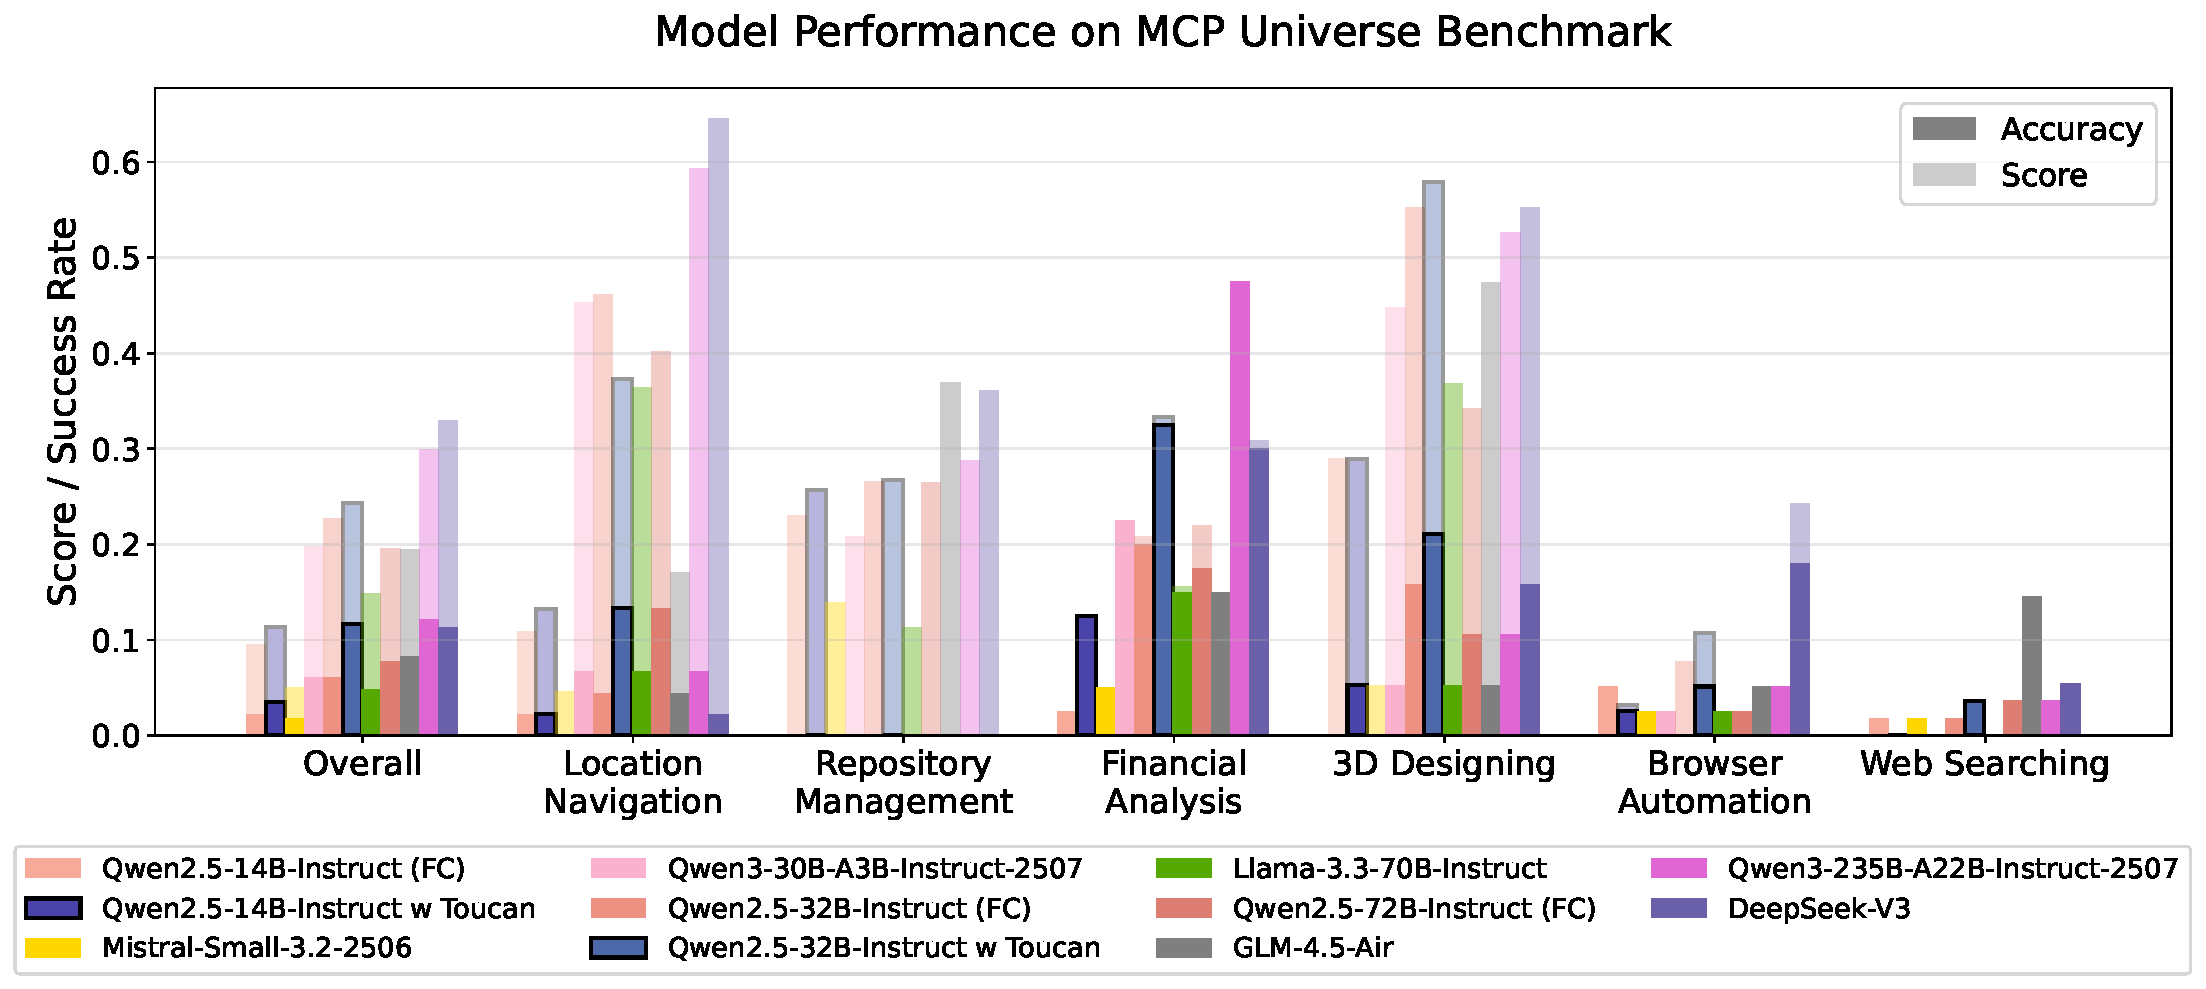
\includegraphics[width=1\linewidth]{images/mcp_universe_bench.pdf}
    \caption{This figure compares the performance of \datanamen-tuned models with other open-source models on MCP-Universe \citep{mcpuniverse}. Model sizes increase from left to right. Bars with darker colors represent task success rate (full task completion), while lighter colors represent average evaluation scores considering partial task completion. \datanamen-tuned models are shown with black borders. \datanamen-tuned models outperform other models of similar sizes across most tasks.}
    \vspace{-1em}
    \label{fig:mcp-universe}
\end{figure}

\begin{wrapfigure}{r}{0.38\textwidth}
  \vspace{-3em}
  \centering
  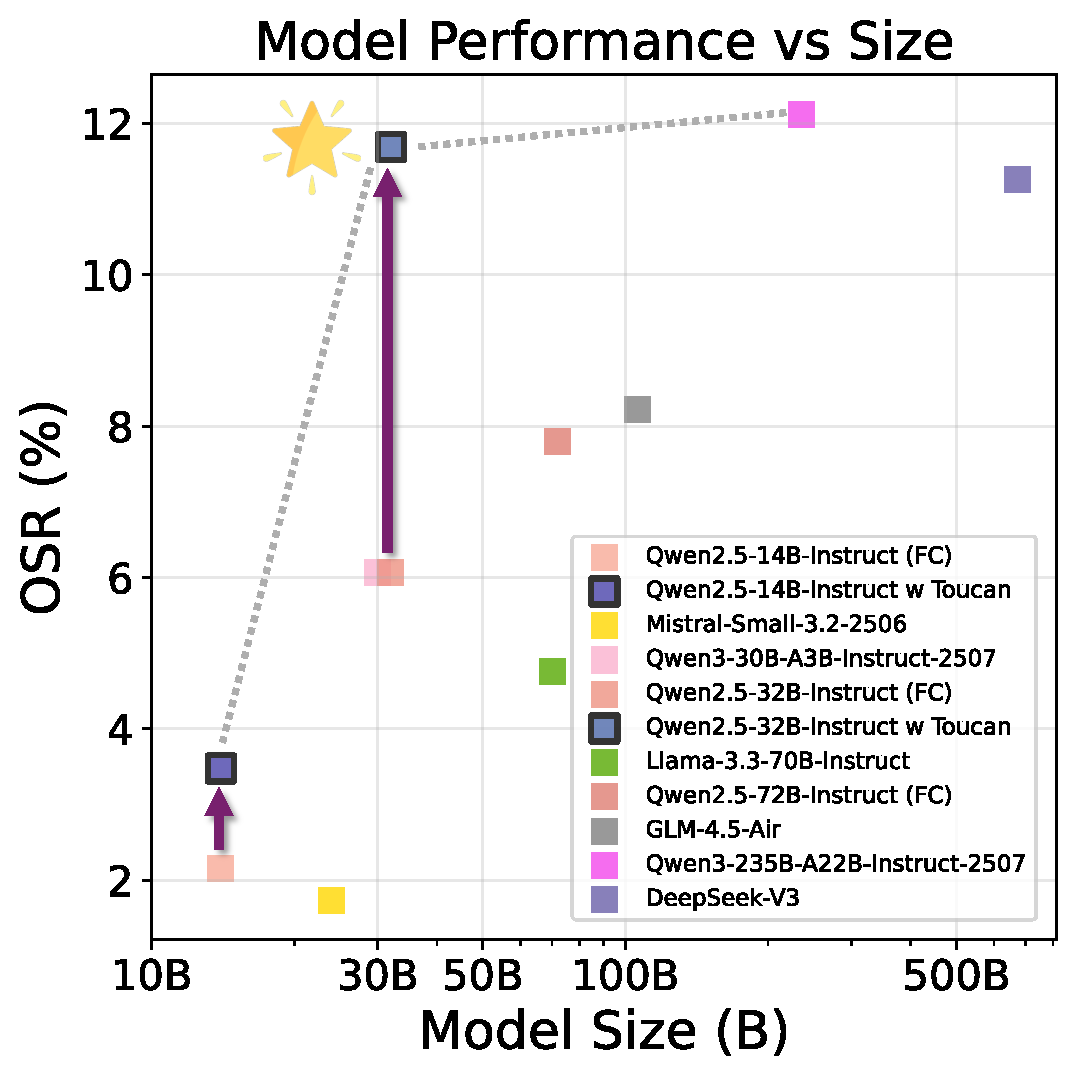
\includegraphics[width=1\linewidth]{images/mcp_universe_model_performance_vs_size.pdf}
  \vspace{-1.5em}
  \caption{Model Performance vs Size on MCP-Universe Benchmark. We report overall task success rate (OSR). Our models push the Pareto frontier forward, achieving higher OSR at smaller model sizes.}
  \label{fig:mcp-universe-pareto}
  \vspace{-2em}
\end{wrapfigure}

\textbf{\dataname Effectively Increases Agentic Tool-Calling Performance.} 
Tables~\ref{tab:bfclv3-results-table} and \ref{tab:tau-results-table} present the experimental results of models fine-tuned on \dataname across BFCL V3, $\tau$-Bench, and $\tau^2$-Bench, respectively. We make the following key observations: 
First, models fine-tuned with \dataname show performance improvements compared to baseline models without fine-tuning across almost all aspects of these three benchmarks, indicating that \dataname effectively enhances the agentic and tool-calling capabilities of models. 
Second, on BFCL V3, models fine-tuned on \dataname outperform larger production LLMs including \texttt{DeepSeek-V3} and \texttt{GPT-4.5-Preview} in average scores and achieve top performance in the \textit{multi-turn} subset. This demonstrates the effectiveness of \dataname and validates our dataset design.

\textbf{\dataname Enhances Models' Performance on Using Real-World MCP Servers.} Figure \ref{fig:mcp-universe} demonstrates a performance comparison between \datanamen-tuned models and other open-source models of similar or larger sizes across six domains: Location Navigation, Repository Management, Financial Analysis, 3D Design, Browser Automation, and Web Search. We note that most servers in the benchmark require careful configurations and thus were not included in our data synthesis pipeline. Nevertheless, \datanamen-tuned models show significant improvements on these challenging tasks compared to baselines, indicating that exposure to diverse tools enhances model performance on agentic tasks. Notably, our 32B model achieves the highest scores in 3D Design and strong performance in Financial Analysis, even outperforming much larger frontier open models like \texttt{Llama-3.3-70B-Instruct}, \texttt{Qwen2.5-72B-Instruct}, \texttt{GLM-4.5-Air} (106B), and \texttt{DeepSeek-V3} (671B).

Figure \ref{fig:mcp-universe-pareto} plots model performance versus model size on MCP-Universe benchmark. We observe that \datanamen-tuned models push the Pareto frontier forward, achieving higher OSR at smaller model sizes, indicating that \dataname can help models achieve superior performance-efficiency trade-offs in agentic tasks.

\subsection{Ablation Analysis}

\begin{wrapfigure}{r}{0.5\textwidth}
  \vspace{-1.5em} % Adjust vertical spacing above the table
  \centering
  \caption{This table shows ablation analysis of \dataname extensions.}
  \label{tab:ablation-results-table}
  \resizebox{\linewidth}{!}{ % Scale to the wrapfigure width, preserving aspect ratio
    \begin{tabular}{@{}lccc@{}}
      \toprule
      & \textbf{BFCLv3} & \multicolumn{2}{c}{\textbf{$\tau$-bench}} \\
      \cmidrule(lr){2-2} \cmidrule(lr){3-4}
      & & \textit{Airline @1} & \textit{Retail @1} \\
      \midrule
      Qwen2.5-14B-Instruct & 57.69\% & 17.25\% & 44.46\% \\
      \quad + Single Turn & 60.16\% & 15.50\% & 36.95\% \\
      \quad\quad + Irrelevance & 64.74\% & 16.75\% & 41.63\% \\
      \quad\quad\quad + Diversify & 64.56\% & 17.25\% & 43.70\% \\
      \quad\quad\quad\quad + Multi-Turn & \textbf{65.09\%} & \textbf{22.00\%} & \textbf{48.48\%} \\
      \bottomrule
    \end{tabular}
  }
  \vspace{-1.5em} % Adjust vertical spacing below the table
\end{wrapfigure}

To validate our extension designs, we perform ablation analysis on the Qwen2.5-14B-Instruct model, where we fine-tune on progressively extended versions of \datanamen, allowing us to isolate the contributions of each extension described in Section \ref{sec:toucan-extensions}. The experimental results are shown in Figrue \ref{tab:ablation-results-table}. We observe that all components contribute to improved scores. Detailed benchmark scores for the BFCL ablation study are provided in Appendix \ref{app:more-on-ablations}.

